\documentclass[fleqn,10pt]{wlscirep}
\usepackage[utf8]{inputenc}
\usepackage[T1]{fontenc}
\usepackage{overpic}

\newcommand{\TODO}[1]{{\bf {\color{red} ToDo:} #1}}

\title{On the Interplay of Clustering, Shortest Path and the Optimal Collective Response}

\author[1,*]{Nikolaj Horsevad}
\author[2,+]{David Mateo}
\author[3.+]{Robert Kooij}
\author[1,+]{Roland Bouffanais}
\affil[1]{Affiliation, department, city, postcode, country}
\affil[2]{Affiliation, department, city, postcode, country}
\affil[3]{Affiliation, department, city, postcode, country}

\affil[*]{nikolajhorsevad@gmail.com}

\affil[+]{these authors contributed equally to this work}

\keywords{Complex Networks, Multi-agent systems, Network structure, Small-World, Scale-Free, Clustering, Path length}

\begin{abstract}

Networked multi-agent systems, both social, natural and engineered, require a good collective response to changes in their environment to operate successfully. The effectiveness of the collective response depends greatly on the topological structure of the interaction network between the agents. We investigate how different network parameters measured on the network topology, affect the collective response, in the leader-follower linear consensus model, where an agent (``the leader'') follows a driving signal. Our analysis has revealed an intricate relationship between the collective response at different frequencies, and network parameters: Path length, Clustering Coefficient and Degree. In a middle range of frequencies, the collective response benefits from a higher clustering coefficient in the network, both for near-regular and scale-free networks, while regular networks experience a higher collective response at low frequencies, when the characteristic path length is low. Further we conduct experiments on a swarm of land robots, conducting an angular consensus algorithm to test our findings, for topologies with a wide range in clustering coefficients. These results greatly help in the design of artificial multi-agent systems, as they shed light on how a static interaction network topology can be made for specific environments, or how a dynamic rewiring topology can tune the system response on the fly. \TODO{Check Abstract}

\end{abstract}
\begin{document}

\flushbottom
\maketitle
% * <john.hammersley@gmail.com> 2015-02-09T12:07:31.197Z:
%
%  Click the title above to edit the author information and abstract
%
\thispagestyle{empty}

%\noindent Please note: Abbreviations should be introduced at the first mention in the main text – no abbreviations lists. Suggested structure of main text (not enforced) is provided below.

\section*{Introduction}

\begin{itemize}
    \item (Motivation) It is known that network structure affects functionality.
    Take a paradigmatic problem in distributed systems: how to achieve global consensus from local interactions.
    \item (Background) The problem of distributed consensus is typically formulated as blah blah.
    It is known that the a successful, global consensus depends on the structure of the interaction network: for instance, consensus is only reached if \ldots and the speed to consensus is proportional to \ldots
    \item (Leader-follower) A common variation of the problem is the leader-follower scheme, where \ldots
    This problem is relevant for (these peoples) and (those peoples).
    \item (Responsiveness) this type of leader-follower consensus problems open up a series of interesting questions, for instance: beyond the capacity of consensus, what can we say about the capacity to adapt the consensus to a dynamic leader?
    \item (Previously on) we have seen that the effects of structure and responsiveness are significantly more complex that the effects on the speed to consensus or such.
    In particular, the degree alone has a nontrivial effect on responsiveness: sometimes less is more and others more is more.
    \item (This work) Here, we study the relation between certain structural properties of the interaction network such as clustering and the characteristic path length and the capacity of a distributed system performing a linear consensus protocol to response to a dynamic signal.
    \item (Conclusion) We observe that X and Y and Z.

\end{itemize}

\TODO{Write introduction}
Why do we explore these things? Structure always affects functionality \cite{strogatz2001exploring}.

The network topology has an impacts a wide range of networked systems  \cite{mateo15:_exces}.

We have already shown the degree has a profound effect \cite{mateo2018optimal}, but as degree changes so does other network parameters, some of the more general ones clustering coefficient and shortest path. Is the degree or the parameters the primary carrier of these gains ?


\section*{Results}


\subsection{Influence of a leader on fully connected graphs}

First, let's consider the case of $N+1$ fully connected agents where one of them is acting as the leader.
In this case, the total response of the system is
\begin{equation}
    H^2 = \frac{N}{1 + (N\omega/\omega_0)^2}
\end{equation}

The maximum total response of such system below the cutoff frequency (i.e. for $\omega \le \omega_0$) is \TODO{Using nondimensional frequencies for some of these, make consistent.}
\begin{equation}
    H^{2^*} = 1 / 2\omega
\end{equation}
for a system size equal to
\begin{equation}
    N^* = 1/\omega
\end{equation}

What this means is that the optimal ``influence sphere'' for a leader trying to drive consensus at a timescale $T=\omega^{-1}$ is directly proportional to the timescale, $N^* = T / T_0$ where $T_0$ is the individual's response timescale.

This $N^*(\omega)$ is such that the cutoff frequency of the system is set to $\omega$.
In other words, the optimal influence sphere of a leader is such that the system operates at its cutoff frequency.


\TODO{Casual mode on.} So, this is the way to optimize $N$ in the case of fully connected graphs.
This does not mean that fully connected is necesarily optimal.
Also, in some cases changing $N$ may not be an option.
Thus, if $N$ is fixed, what is the best we can do? Let's see\ldots

\subsection{Optimal response in small-world networks}

To study how the properties of the interaction network affect the collective response, we focus our attention first on the classic Watts-Strogatz small-world network model.
This model allows us to explore, by changing a single parameter $p$, three different regimes: a high clustering, high path one (ring)regime, a high clustering, low path one (small-world), and a low clustering, low shortest path (random).

Figure XX shows the collective response in a WS network for different values of the switching probability $p$.
This results show that the system depends three different regimes depending on the frequency:
\begin{itemize}
    \item Low frequency ($\omega < 0.01$): the response monotonically increases with $p$.
    This suggest that, at low frequencies, having a small path is paramount for a good response. \TODO{Maybe it is the lack of clustering that helps, thats why we also need the MHK}
    \item Mid frequencies ($0.01 < \omega > 1$): the response monotonically decreases with $p$.
    This suggest that, at mid frequencies, having a high clustering is paramount for a good response.
    \item Large frequencies ($\omega > 1$): the response is independent of $p$.
    This result is to be expected, as at very high frequencies the response of this system is independent of the structure of the network beyond its average degree $k$ (see \cite{mateo15:_exces}).
\end{itemize}

Note that at no frequency is the finite $p$ values corresponding to a small-world optimal.
In other words, there does not seem to be any range of frequencies at which it is important to have both clustering and path.


\subsection{Evolved networks}


\subsection{STUFF TO BE MOVED TO THE PROPER PLACE}

We have previously shown that networked systems with widely different networkg topologies are able to maximize the collective response by tuning the average degree of the network nodes \cite{mateo15:_exces}\cite{mateo2018optimal}. But as the degree distribution varies, many other charachteristics, such as clustering and average path length, of the network structure can vary in nontrivial ways.

Figure \ref{fig:gaincmp} shows the collective response, $H^2(\omega)$ to a single leader oscilating with frequency $\omega$, for different network topologies with $N+1= 257$ agents following the linear consensus of \ref{eq:dynamic}. The insert (C) shows how the mean network degree changes with the freqyency such that $H^2(\omega)$ has $k(\omega) = k*(G,\omega)$. The nontriviel changes that occurs in the clustering, $CC$ and the average shortest path length, $SP$ as $k*$ changes are shown on the side in (D) and (E) .

 For systems with $N =  257$ nodes, the optimal response and the optimal degree $k^*$ varies in different ways between a low frequency $\omega_{low} \approx 0.004$ and a high frequency $\omega_{high} \approx 1.3$, but outside of these frequencies all network models either have $k=k_{max}$ or  $ k=k_{min}$ for their respective models. The insert in Figure \ref{fig:gaincmp} shows how the transitioning from low to high frequency has a different number of steps for different network topologies, where it seems that networks that are highly clustered topologies have a better collective response.
% , see  table~\ref{tab:ccsp}, and a wider range of optimal connectivity's.

\begin{figure}[!b]
\begin{overpic}[unit=1mm,scale=.78]{fig/gaincmp.pdf}
  \put(40,72){\large(A)}
  \put(40,30){\large(B)}
  \put(60,72){\large(C)}
  \put(60,47){\large(D)}
  \put(60,22){\large(E)}
\end{overpic}
\caption{A) Collective response for the regular lattices with $N=257$ agents, and different average degree. B) Collective response at optimal degree $k^*$, for different network topologies, with system size $N=257$, ($N = 240$ for the caveman network, $N=240$ for the clique network). C) for differed  topologies. D) Network clustering for a given $k^*$. E) Network characteristic path length for a given $k^*$ (in clique network this is infinite due to disconnected cliques).}
\label{fig:gaincmp}
\end{figure}




Figure~\ref{fig:wscmp} shows the collective response $H^2(G_{\textsc{WS}}(k^*(\omega),p))$ for network topologies generated by the Watts Strogatz model, with system size of $N = 257$, at the optimal degree $k^*$. For low and high frequencies above $\omega = 0.005$ or below $\omega = 0.2$ the changes in $p$ incurs no noticeable difference in the collective response, or the values of $k^*$, see Figure~\ref{fig:wscmp} insert. In the frequencies between $\omega_{low}$ and $\omega_{high} $ the collective response shows a decrease as $p$ increase. This decrease in the maximum collective response is mirrored in a decreased range of $k* \neq\{k_{max}, k_{min}\}$, which decreases as $p$ increases. Here $k^*(p,\omega)$ moves from being like the ring network, to that of a random network, with intermediate steps as $p$ increases. Keep in mind as $p$ increases, the clustering decreases.

\begin{figure}[hbtp]
  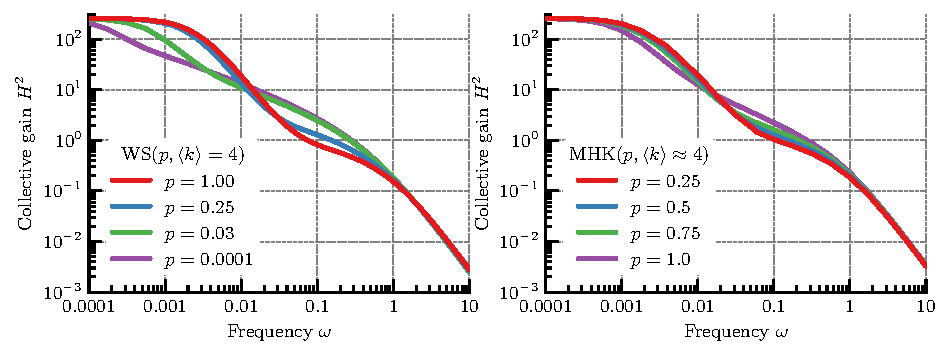
\includegraphics[width=0.997\textwidth]{fig/ws_mhk_response.pdf}
\caption{Differences in the watts strogatz model networks and the modified Holme kim models for different values of $p$. As p increase in MHK clustering does too, in the Watts strogatz it is opposite. All networks have an average degree of $\langle k\rangle =4$. The result is the average of $200$ model runs for each value of $p$. \TODO{maybe make an insert of a historgram with the degree distribution??}}
%\caption{Frequency response at the optimal connectivity, $k*$ for Watts Strogatz Small World networks, with system size $N=256$. Insert: the optimal connectivity $k*$ in Watts Strogatz small world networks, as a function of frequency.}
\label{fig:wscmp}
\end{figure}


% \begin{figure}[hbtp]
%   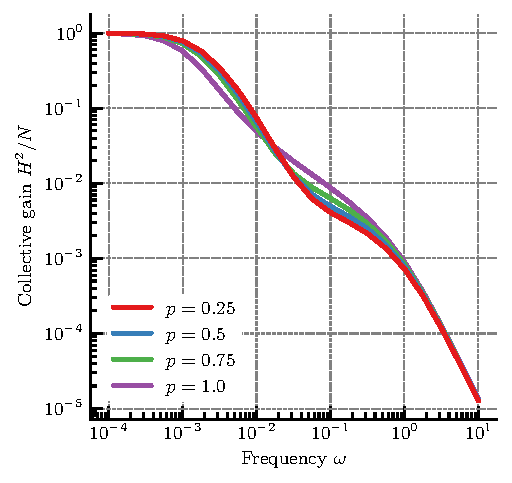
\includegraphics[width=0.9\textwidth]{fig/mhk_cmp.pdf}
% \caption{Frequency response at the optimal connectivity, $H^2(\omega)$ for the modified Holme Kim model, with system size $N=256$. The average degree approches $\langle k\rangle = 4$. It is visible how at medium frequencies }
% \label{fig:mhkcmp}
% \end{figure}



As it is difficult to decouple elements of the network structure from each other, Figure~\ref{fig:prop_cmp} shows a comparison of the degree, average shortest path and average clustering coefficient for a range of networks generated with the Watts Strogatz model, with $257$ agents. Each row in Figure\ref{fig:prop_cmp} is at a specific frequency, and each column shows the different network properties, average degree, average shortest path, average clustering. All the variability in the networks comes from changing $p$ in the Watts Strogatz model. Firstly in column one, it can be seen that the optimal gain for a given frequency moves to a lower degree $k$ as the frequency increases, as would be expected from out last paper \TODO{reff}. Here is is also shown that the variability in the gain is larger in low degree networks compared to high degree networks, this is due to more re-configurations being possible with a lower number of connections in the network. At low frequencies any degree $k$ can get close to the maximum performance, but as the frequency increases, the differences in maximum gain at a given degree $k$ increase. When looking at the average shortest path column, an almost linear relationship is seen between the average shortest path length and the gain. This shows that as the shortest path decrease, the gain increase, to the point at $\min({SP(k))})$ the gain is the same independently of the $k$. At low frequency there does not seem to be any correlation between the clustering and the gain.
When the frequency is high on the other hand, there seems to be a relationship between the clustering and the gain, where the gain increases as the clustering increases. Somewhere in between the maximum collective response for a given connectivity $k$, changes from happening at the lowest average shortest path, to the highest average clustering. It is shown in the middle row, how this change occurs at different frequencies for different connectivity's, as the highest gain for $k=32$ happens at a average shortest path of $2$ and average clustering of $0.1$ \TODO{check the numbers}, where for a connectivity of $k=8$ the maximum gain is at average shortest path of $18$ and clustering of $0.7$ \TODO{Check numbers}.



As $\omega$ increases $H^2$ decreases.
At mid $\omega$, the optimal setting, low $SP$ or high $CC$ might be best, this also depends on the degree $k$



\begin{figure}[hbtp]
  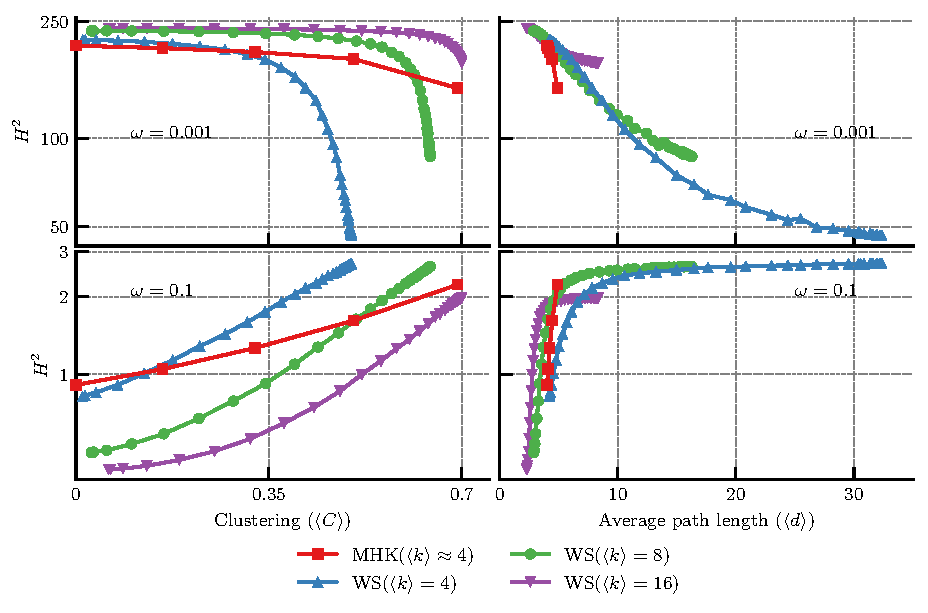
\includegraphics[width=0.95\textwidth]{fig/prop_cmp.pdf}
  \caption{Gain data for the Watts Strogatz small world model with $p$ between $0$ and $1$, where the grid rows have different frequencies, and the columns represent different network quantities on the x-axis. The plots are colored after their mean degree$<k>$. In the first column it can be seen how $k^*$ decrease as the frequency increases. The second column show how the networks collective response changes with the average shortest path, notice that almost linear relation at low frequencies, and that a smaller shortest path always is beneficial. The third column, show how the collective response changes with the clustering, notice the collective response gets better with higher clustering as the frequency goes up. In the middle row of columns two and three it can be seen that the preference in the network for high clustering or low shortest path for the highest collective response is different at high and low $k$, which indicate that not only does the gain depend on the network structure, but this varies both with frequency and overall degree distribution. \TODO{Make the points not based on average $CC$ for a value of $p$, but bin them according to $CC$ value and then replot},\TODO{Change the values of $k$ from 4 to 32 instaead, it is hard to distinguish the top panels with k=4 for such a large range}}
\label{fig:prop_cmp}
\end{figure}


\subsection*{Experimental validation}

\begin{figure}[hbtp]
  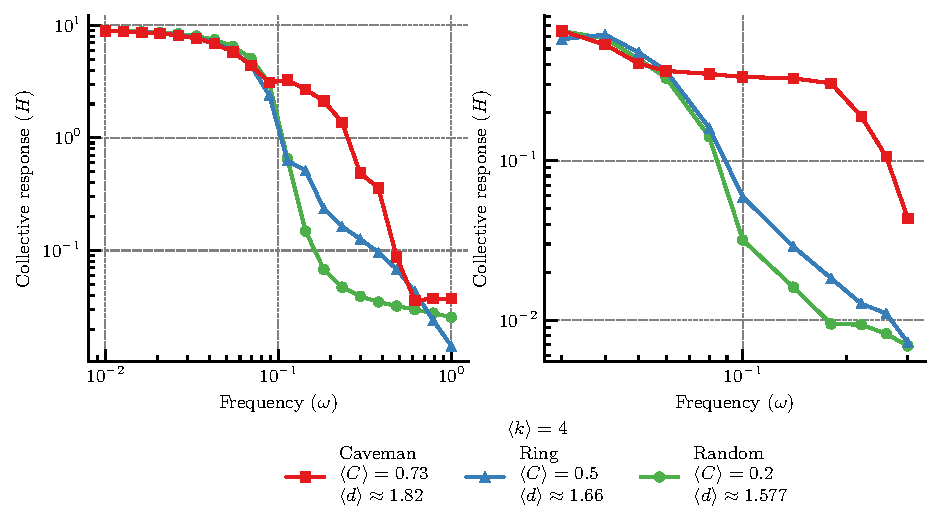
\includegraphics[width=0.9\textwidth]{fig/sim_exp.pdf}
\caption{The simulated and experimental results of 10 agents preforming angular consensus on the ring, caveman and a random regular communication graphs. This shows that the caveman graph is superior in the medium frequencies, but has the same performance at high and low frequencies at the other networks, both for the simulated results, and the experiment. }
\label{fig:exp_sim}
\end{figure}


% \begin{figure}[hbtp]
%   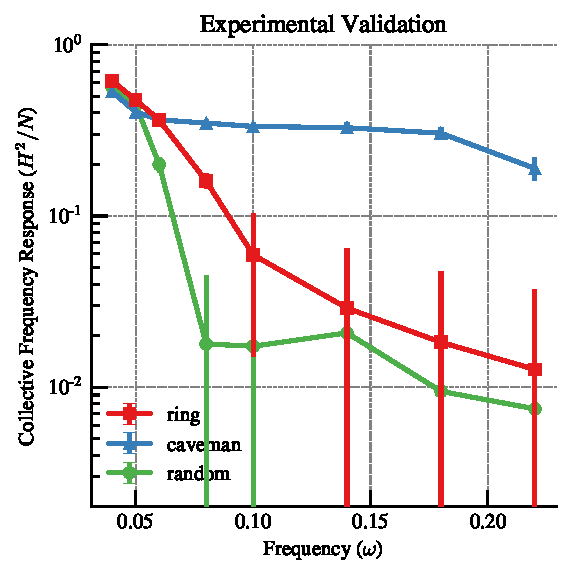
\includegraphics[width=0.9\textwidth]{fig/experimental_gain.pdf}
% \caption{Experimental collective responses for the networks simulated. These are consistent with all other findings that clustering is a very desirable property at the medium frequency range. Due to the small network size, it is difficult to observe any benefits from the shortest path at low frequencies.}
% \label{fig:exp_res}
% \end{figure}

\subsection*{Optimization}

Put some results for the genetic algorithms

\begin{figure}[hbtp]
  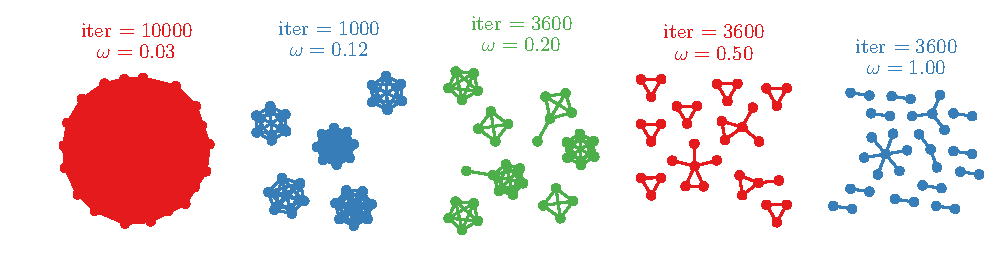
\includegraphics[width=0.9\textwidth]{fig/ea_graph.pdf}
\caption{Graphs as they evolve in the evolutionary algorithm}
\label{fig:ea_graph}
\end{figure}



\TODO{Beautiful results, that can convince people how amazingly good we are at science}



\section*{Discussion}

In the low frequency regime, that is until $k*$

\TODO{The amazing results, clearly indicating that we are awesome scientists}



\section*{Methods}

\section*{Eigenvalues and the Graph matrices}
For Regular graphs we have the relation that $k - \lambda(A) = \lambda(L) = \frac{1}{k}\lambda(L_{rw})$
\subsection*{Adjecency matrix}
The adjacency matrix is $A$.

\begin{align}
  \sum_{i=0}^{N} \lambda_i &= \mathrm{\text{number of self-loops  in }}G \\
  \sum_{i=0}^{N} \lambda_i^2 &= 2 \times \mathrm{\text{number of edges in }}G \\
  \sum_{i=0}^{N} \lambda_i^3 &= 6 \times \mathrm{\text{number of triangles in }}G
\end{align}

These properties seen in the equation above are very interesting, if we consider some k-regular graphs with the same number of nodes, like a k-regular random, circular and caveman graph, as the sum of squared eigenvalues will be the same, but the sum of cubes will not. Further the number of triangles are direcyly related to the Clustering and transitivity of the network (which are almost equal in Watts-Strogatz random networks, and then I assume also in these k-regular networks.) The transitivity can be calculated as 
\begin{equation}
  C = \frac{\operatorname{trace}A^3}{\sum_{i \neq j} (A^2)_{i,j}} =  \frac{\sum\lambda_i^3}{\sum_{i \neq j} (A^2)_{i,j}} 
\end{equation}

This come from the x, power of the adjacency maktrix gives the number of paths of length x between two nodes, eg. power 3 of adjacency matrix, gives the mumber of triangles on the diagonal. 

The largest eigenvalue of the adjacency matrix is a "sort" of measure of the average degree of the graph. Especially if the graph is $k$-regular, this eigenvalue will be $k$.  Thus for a $k$-regular graph, the largest eigenvalue of the adjacency matrix $
\lambda_{max} = k$. This translates to the 0 eigenvalue of the Laplacian graphs, as $k-\lambda_{max}(A) = \lambda_1(L) =  \lambda_1(L_{rw}) = 0$.  For more general graphs, the eigenvalue is bounded by $\max(\bar{k},\sqrt{k_{max}}) \leq \lambda_{max}(A) \leq k_{max}$ where $\bar{k}$ is the average degree on the graph. 



\subsection*{Laplacian matrix}
The Laplacian matrix $L$ is given as $L = D-A$ where the Degree matrix $D(G)$ is assumed ordered so the collums correspond to the vertices in the graph $G$, and the diagonal entried are $d_i$. 

We also have that the algebraic connectivity, which is analogous to the shortest path (I think), is the second smallest eigenvalue of the the laplacian. What is interesting is that both the optimization done by David and Nikolaj show that at medium frequencies (The range whete $k^*$ is no longer $k_{\text{max}} $) crates disconnected networks, where $\lambda_2$ will be 0. This is due to the multiplicity of the 0 eigenvalue is equal to the number of connected components of the graph, thus a disconnected graph will have $\lambda_2 = 0$. This might be another way of explaining why we have to look beyond $\lambda_2$, when we introduce a time varying dynamics into the system.

\subsection*{Random-walk Laplacian matrix}
The Random-walk Laplacian is the matix is given as $L_{rw} = D^{-1} L$. The matrix $L_{rw}$ is equal to the system matrix, when the Graph describes the network used by a number of nodes to preform the classical LTI-consnsus algorithm.  How does the eigenvalues change when we introduce a leader ? ?.
In the ring network $L_{rw}(G)$ of a graph where one node has been taken out to be the leader, is the same as the $L_{rw}(G)$ with 1 less nodes. This might be helpfull in doing analysis on this

\section*{Methods}\label{sec:Methods}

\subsection*{Distributed Linear Consensus}
\label{sec:dlc}

Consider a set of $N + 1$ identical networked agents preforming a distributed consensus algorithm on a scalar state variable $x_i(t)$. The system dynamics are determined by the state vector $\mathbf{x}(t) = \{x_{0}(5),x_{1}(t),\ldots,x_{1}(t) \}$ and the communication graph between the agents, described by an adjacency matrix $\mathbf{A}$, with elements $a_{ij} = 1$ if a connection exists from agent $i$ and $j$ and $a_{ij} = 0$ otherwise. With a specific network topology the system evolves as

\begin{equation}
  \label{eq:lincon}
  \frac{dx_i}{dt} = \frac{\omega_0}{k_i} \sum^{N}_{j = 0} a_{ij} (x_i(t)) - x_j(t)),
\end{equation}

where $k_i = \sum_{j=0}^N a_{ij}$ is the degree of agent $i$, $\omega_0$ is the natural response frequency of the agents. This can be written compactly by collecting terms in a single weight $w_{ij} = \frac{\omega_0}{k_i} - \delta_{ij}$, with $\delta_{ij}$ as the Kronecker delta function, yielding
\begin{equation}
  \label{eq:consht}
  \frac{dx_i}{dt} = \sum^{N}_{j = 0} w_{ij} (x_j(t)).
\end{equation}

In order to model the collective response, consider an agent with privileged information, the ``leader'', say agent $i=0$. The leader does not follow the consensus dynamics of eq.~\ref{eq:consht} but rather some  arbitrary trajectory $x_0(t) = u(t)$. Given this leader, the dynamics changes to

\begin{equation}
  \label{eq:dynamic}
  \frac{dx_i}{dt} = \sum^{N}_{j = 1} w_{ij} (x_j(t)) + w_{i0}u(t))
\end{equation}

for the follower agents $i=1,2, \dots, N$. This can be put on matrix form as

\begin{equation}
  \label{eq:dynmat}
  \frac{dx}{dt} = W_Fx(t)  + W_Lu(t).
\end{equation}

The system response, can then be found by the ability of the follower agents to follow the leaders trajectory. When the leaders trajectory is an oscillating input signal $u(t)=e^{j\omega t}$, at frequency $\omega$, the steady state response of all agents becomes proportional to this input signal. This response can be found by taking the Laplace transform of eq.~\ref{eq:dynmat} and finding the transfer function

\begin{equation}
  \label{eq:contf}
  H(\omega) = \lim_{t \to \infty}\frac{x(t)}{u(t)} = \left(j\omega I - W^{l}_F\right)^{-1}W^{l}_L,
\end{equation}
where $I$ is the $N\times N$ identity matrix, $W^{l}_F = \{w_{ij}\}$ is the consensus protocol matrix between the follower agents with leader $l$, $W^{l}_L = \{w_{i0}\}$ is the consensus protocol matrix between the followers and the leader agent $l$, and $H(\omega)=\{h^{l}_i\}$ is a $1 \times N$ vector where the element $h^{l}_{i}$ is the response of follower agent $i$ to the leader agent $l$ input signal. It should be noted that the response in eq.~\ref{eq:contf} has an intricate relationship with the underlying communication graph. To quantify the ability of the system as a whole to respond to the leaders input, the collective response for a leader is defined as
\begin{equation}
H^{2}(\omega) = \frac{1}{N}\sum_{j=0}^{N}\sum_{i\neq j}|h_i^j(\omega)|^2.
\label{eq:colgain}
\end{equation}
We average over all agents as the leader in the networks that do not contain homogeneous agents, such as random graphs, Watts Strogatz, caveman graphs, where the collective response would otherwise depend on the leader placement in the network.

\subsection*{Network analysis}
\label{sec:na}

To characterize the networks we focus on the average degree $\bar{k} =  \sum_{i=0}^{N}k_i$, the average local clustering coefficient $\bar{C}$ and the characteristic path $\bar{L}$ as defined in \cite{watts1998collective}.

\subsection*{correlations}      

The correlations are calculated using the spearman rank corrlation, where the variabels $(X,Y)$ are ranked from low to high as $(rX,rY)$ and the correlation is calculated on the ranked values instead:
\begin{equation}
Corr = \frac{\operatorname{cov}(rX,rY)}{\sigma(rX)\sigma(rY)}
\end{equation}
In the case of the variables having the sane rank in the set, they are assigned fractions of their respective rank, eg. 2 elements of $X$ have the lowerst set values of 1, they are both assigned a rank of $0.5$

\subsection*{Network models}


\subsubsection*{Connectivity Network models }

\paragraph{$k$-Regular Lattice}
The regular lattice graphs are constructed by placing the agents in a grid with periodic boundaries, and connecting each agent to the $k$ nearest neighbors on the grid. This network structure creates homogeneous agents, where all network parameters are the same. To keep the symetry on the graph, the agents degree is restricted to even numbers from $2$ to $N$.  These networks are highly clustered with a medium network diameter.

\paragraph{Connected Caveman graph}

The caveman graph of size $N$ consist of $n$ cliques, which are complete subgraphs, with the exception of a single edge that is moved from between two agents in the clique, to connect with the neighboring cliques, insuring a connected graph. The caveman graph is the most clustered sparse graph there is \cite{Watts99}, with an average degree of $k$, only having having two agents with $k + 1$ and  $k-1$ respectively, in each clique, and all other agents have a degree of $k$. Due to the graphs being organized in cliques it is not possible to choose an abritray degree for a network of $N$ agents, because it must satisfy that $N=n(k+1)$, therefore $N$ will be choose as a highly composite number.

\paragraph{Regular random networks}

We also consider the regular random graphs, which are sampled from the $k$-regular graphs with $N$ nodes. These graphs are expected to have less structure in them, meaning lower shortest path and clustering coefficient. \TODO{ref}. Unless otherwise stated, results for random graphs are obtained from averaging over 100 realisations.

\TODO{put table with approximate clustering and shortest path ??}

\paragraph{Watts Strogatz small-world}

To study the collective response for a wide range of clustering and shortest path pairs, we consider the Watts Strogatz small-world model~ \cite{watts1998collective}, which rewires the edges in a regular lattice with some probability $p$. Thereby it is possible to create networks with an almost uniform degree distribution, that lie between the regular lattice and the regular random networks. These graphs enable us to study the region of graphs with low shortest paths and high average clustering..


\paragraph{Modified Holme Kim model}
We also consider the Modified Holme Kim model (MHK) to study the effects of clustering and shortest paths in scale free networks. The graphs are constructed from an initial regular lattice of 4 agents, each with a degree of $k=2$. New nodes are then introduced to the graph, where they are connected with two edges to the original structure. The edges are connected to a pair of neighboring agents, such that a triangle is formed, with probability $p$, otherwise it connects to two non-neighboring agents. This will either increasing or decreasing the average clustering coefficient in the network. In the limit, the average degree is  $\lim_{ N\to \infty} \langle k \rangle = 4$, and the clustering is between $0.7$ and $0$~\cite{sekunda16:_inter}.


\subsection*{Network Optimization}

Genetic algorithms, individuals is the adjacency matrix $A$, with $a_{ij} = {0,1}$. We only deal with simple graphs so for efficiency we only use the upper triangular part of the adjecency matrix. On each generation individuals has a probability to mutate, where approximately 2-3 elements in the adjacency matrix change value. On each generation two individuals can be mated, where the nodes between two indices, with all their entries in the adjacency matrix are exchanged, between the two individuals. The fitness of a graph is measured by the collective response for the network graph as described in eq~\ref{eq:colgain}
\TODO{Make note on evolutionary algorithm stuff}


Genetic algorithms. RESULTS: This produces disconnected networks of cliques around the size of what the disconnected caveman network gives.



\subsection*{Experimental setup}
\label{sec:exp}

To imperically measure the collective response of a robotic swarm we have conducted leader-follower heading consensus experiments using 10 robots as in \TODO{cite previous paper}. One of the 10 eBots acts as the leader, where it does not follow the consensus protocol, instead it is continiously adjusting its heading, and rotating at a constant frequency $\omega$. The 9 other robots follow a heading consensus protocol, where they also recieve the heading of the leader, without any way of distinguishing the leader from the other robots. The 9 follower robots follow their own heading $\bar{\theta}$ determined by the consensus protocol
\begin{equation}
  \label{eq:ang_mean}
  \bar{\theta_i} = \langle \theta_j\rangle_{j \sim i} = \arctan \left(\frac{\sum_{j \sim i} \cos\theta_j}{\sum_{j \sim i} \sin{\theta_j}}\right),
\end{equation}

where $j\sim i$ is the neighbors of $i$ and $\langle \cdot \rangle$ is the angular mean. The follower robots update their target heading asynchronously at $\Delta T = \SI{0.1}{\second} $  The information of a robots state is also broadcast to the others at an interval of $\SI{0.1}{\second}$ but not nessesarily concurrently with eachother or the robot. The experiment is preformed with the three static network topologies described in~\ref{sec:nm}. The collective gain of a single agent $i$ following the leader $l$

\begin{equation}
\label{eq:ang_con}
H^l_i = \frac{1}{T}\int_0^T \cos(\theta_i - \theta_l) dt
\end{equation}

\section{Complex Contagion Correlations}

Here are the results of our complex contagion, and how it resembles the results from the Linear Consensus Model.

\begin{figure}[hbtp]
  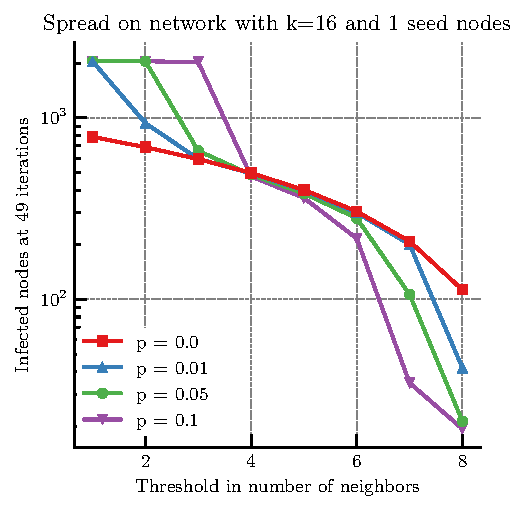
\includegraphics[width=0.997\textwidth]{fig/response_ws_2048_16_1.pdf}
\caption{Watts strogats model for network, high $p$ low clustering, low $p$ high clustering. Linear threshold model, seeded with 1 node, and all its neighbours being infected, letting simulation run for 49 iterations. }
\label{fig:wscmp}
\end{figure}

\begin{figure}[hbtp]
  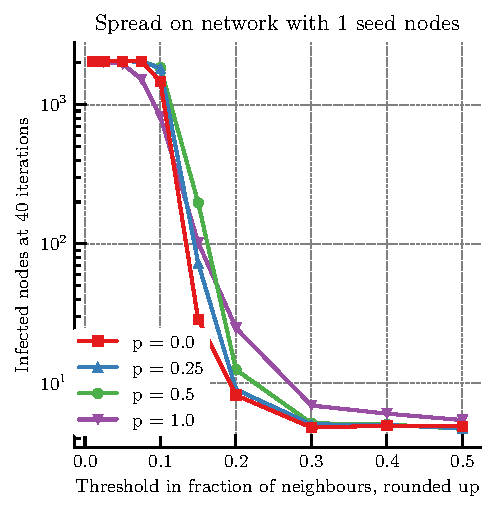
\includegraphics[width=0.997\textwidth]{fig/2048_1_response.pdf}
\caption{Modified holme Kim network mode, low $p$ low clustering, high $p$ high clustering. Linear threshold model, seeded with 1 node, and all its neighbours being infected, letting simulation run for 40 iterations. }
\label{fig:wscmp}
\end{figure}

\newpage
\section{Correlation Results}
To corroborate that indeed the clustering, shortest path, and degree all play a determinant role in the system's response at different frequencies, Fig.~\ref{ws_correlation} shows the correlation between these parameters and the response for a large number of explored networks. It is important to remember that a good correlation is the absolute value of the correlation number, so 1 and -1 are equally strong correlations, just in opposite directions.

\begin{figure}[H]
    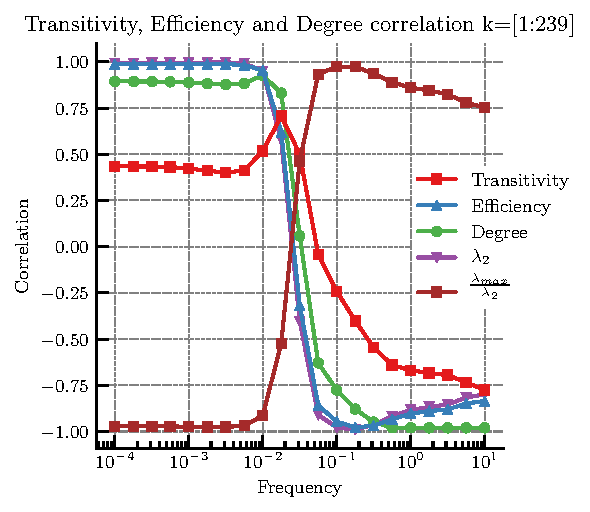
\includegraphics[width=0.8\linewidth]{fig/Transitiviry_Efficiency_DEgre_correlation_ALL}
    \caption{Correlation for networks of types, Watts Strogatz, MHK, caveman, connected\_caveman, with $k$ ranging from 2 to 239, all networks have 240 nodes.}
    \label{ws_correlation}
\end{figure}

Due to the interplay between clustering and degree (hypothesis, you want to maximize clustering, while also decreasing the degree in the middle frequency range), there is an advantage to limit the range of degrees considered in the correlation results. When the number of considered degrees is smaller, the correlation with the clustering becomes stronger in the mid frequency range, see~\ref{ws_correlation_less}.

\begin{figure}[H]                             
    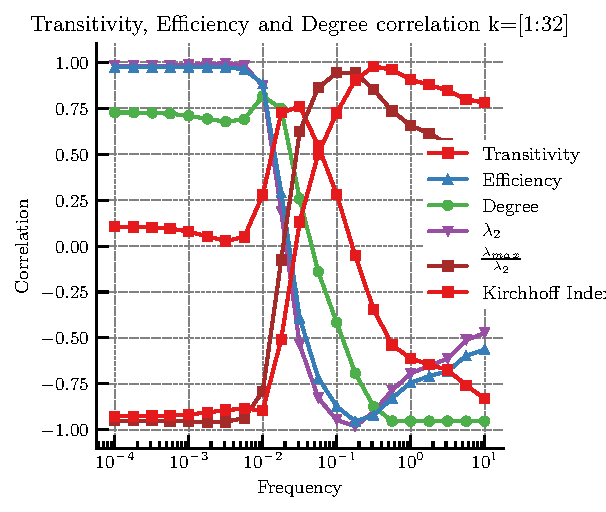
\includegraphics[width=0.8\linewidth]{fig/Transitiviry_Efficiency_DEgre_correlation_1_32}
    \caption{Correlation for networks of types, Watts Strogatz, MHK, caveman, connected\_caveman, with degree $(k)$ of [4,8,16,32] all networks have 240 nodes.}
    \label{ws_correlation_less}
\end{figure}

We can  also consider the correlation for a single degree. In doing so we loose the degree correlation int he graphs, but we get a clearer view of the clustering results, as these are not conflated with the changing degree. See~\ref{ws_correlation_4} for $k=4$, ~\ref{ws_correlation_8} for $k=8$, ~\ref{ws_correlation_16} for $k=16$, ~\ref{ws_correlation_32} for $k=32$, 

\begin{figure}[H]
    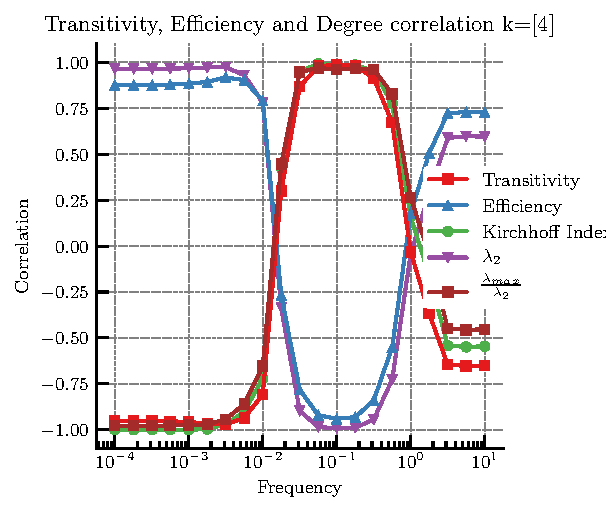
\includegraphics[width=\linewidth]{fig/Transitiviry_Efficiency_DEgre_correlation_4} 
    \caption{Correlation Watts Strogatz and MHK networks $k=4$ all networks have 240 nodes.}
    \label{ws_correlation_4}
\end{figure}

\begin{figure}[H]
    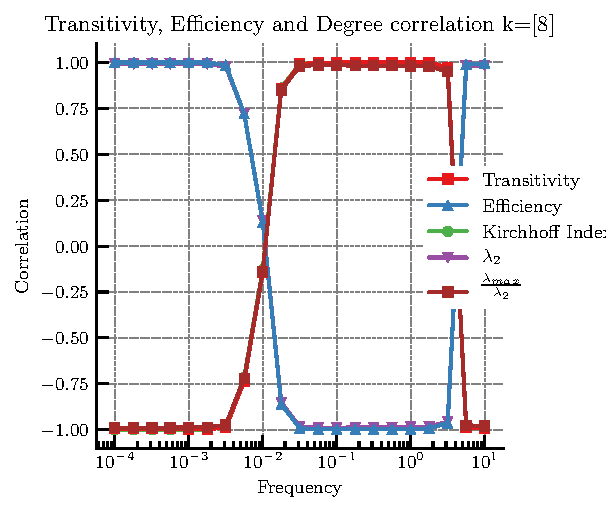
\includegraphics[width=\linewidth]{fig/Transitiviry_Efficiency_DEgre_correlation_8.pdf} 
    \caption{Correlation Watts Strogatz networks $k=8$ all networks have 240 nodes.}
    \label{ws_correlation_8}
\end{figure}

\begin{figure}[H]
    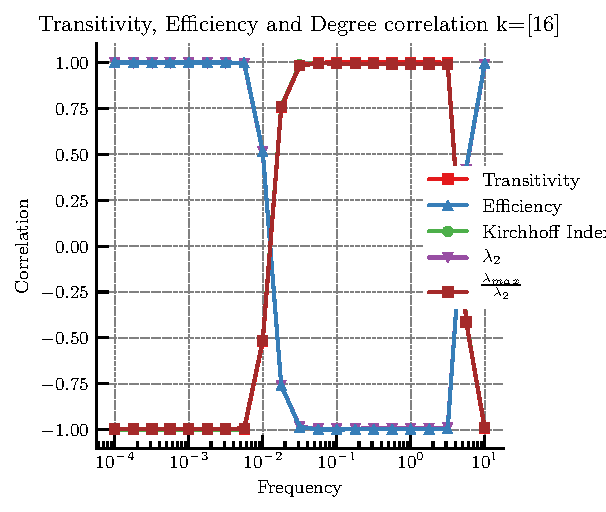
\includegraphics[width=\linewidth]{fig/Transitiviry_Efficiency_DEgre_correlation_16.pdf} 
    \caption{Correlation Watts Strogatz networks $k=16$ all networks have 240 nodes.}
    \label{ws_correlation_16}
\end{figure}

\begin{figure}[H]
    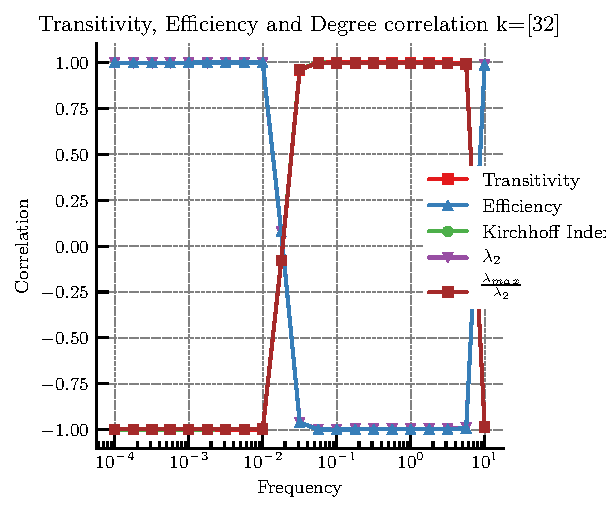
\includegraphics[width=\linewidth]{fig/Transitiviry_Efficiency_DEgre_correlation_32.pdf} 
    \caption{Correlation Watts Strogatz networks $k=32$ all networks have 240 nodes.}
    \label{ws_correlation_32}
\end{figure}

\subsection{Betti numbers}
Betti numbers are numbers used in topology, to describe diffent shahpes. They can also be used to compare graphs, where graphs with similar betti numbers will have some similar structure. Conceptually Betti numbers code for holes in different dimensions. The correlatin with the first 4 betti numbers are seen in~\ref{ws_betti_correlation}. However these are interesting metrics, they do not provide any advantage over previously explored metrics, and the computation of the betti numbers is very demanding, which makes generally unsuitable to this research.

\begin{figure}[H]
    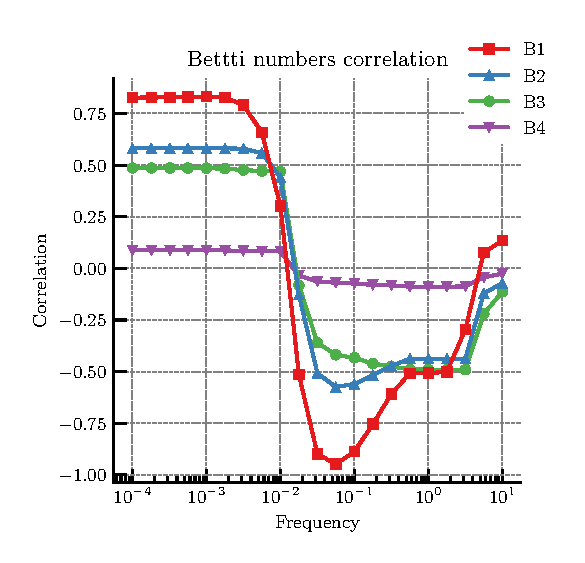
\includegraphics[width=0.8\linewidth]{fig/betti_correlation}
    \caption{Correlation Watts Strogatz networks  $k$ ranging from 2,16, all networks have 240 nodes.}
    \label{ws_betti_correlation}
\end{figure}


\bibliography{biblio.bib}

For data citations of datasets uploaded to e.g. \emph{figshare}, please use the \verb|howpublished| option in the bib entry to specify the platform and the link, as in the \verb|Hao:gidmaps:2014| example in the sample bibliography file.

\section*{Acknowledgements (not compulsory)}

Acknowledgements should be brief, and should not include thanks to anonymous referees and editors, or effusive comments. Grant or contribution numbers may be acknowledged.

\section*{Author contributions statement}

Must include all authors, identified by initials, for example:
A.A. conceived the experiment(s),  A.A. and B.A. conducted the experiment(s), C.A. and D.A. analysed the results.  All authors reviewed the manuscript. 

\section*{Additional information}

To include, in this order: \textbf{Accession codes} (where applicable); \textbf{Competing interests} (mandatory statement). 

The corresponding author is responsible for submitting a \href{http://www.nature.com/srep/policies/index.html#competing}{competing interests statement} on behalf of all authors of the paper. This statement must be included in the submitted article file.

\end{document}